\begin{figure*}[t]
    \centering
    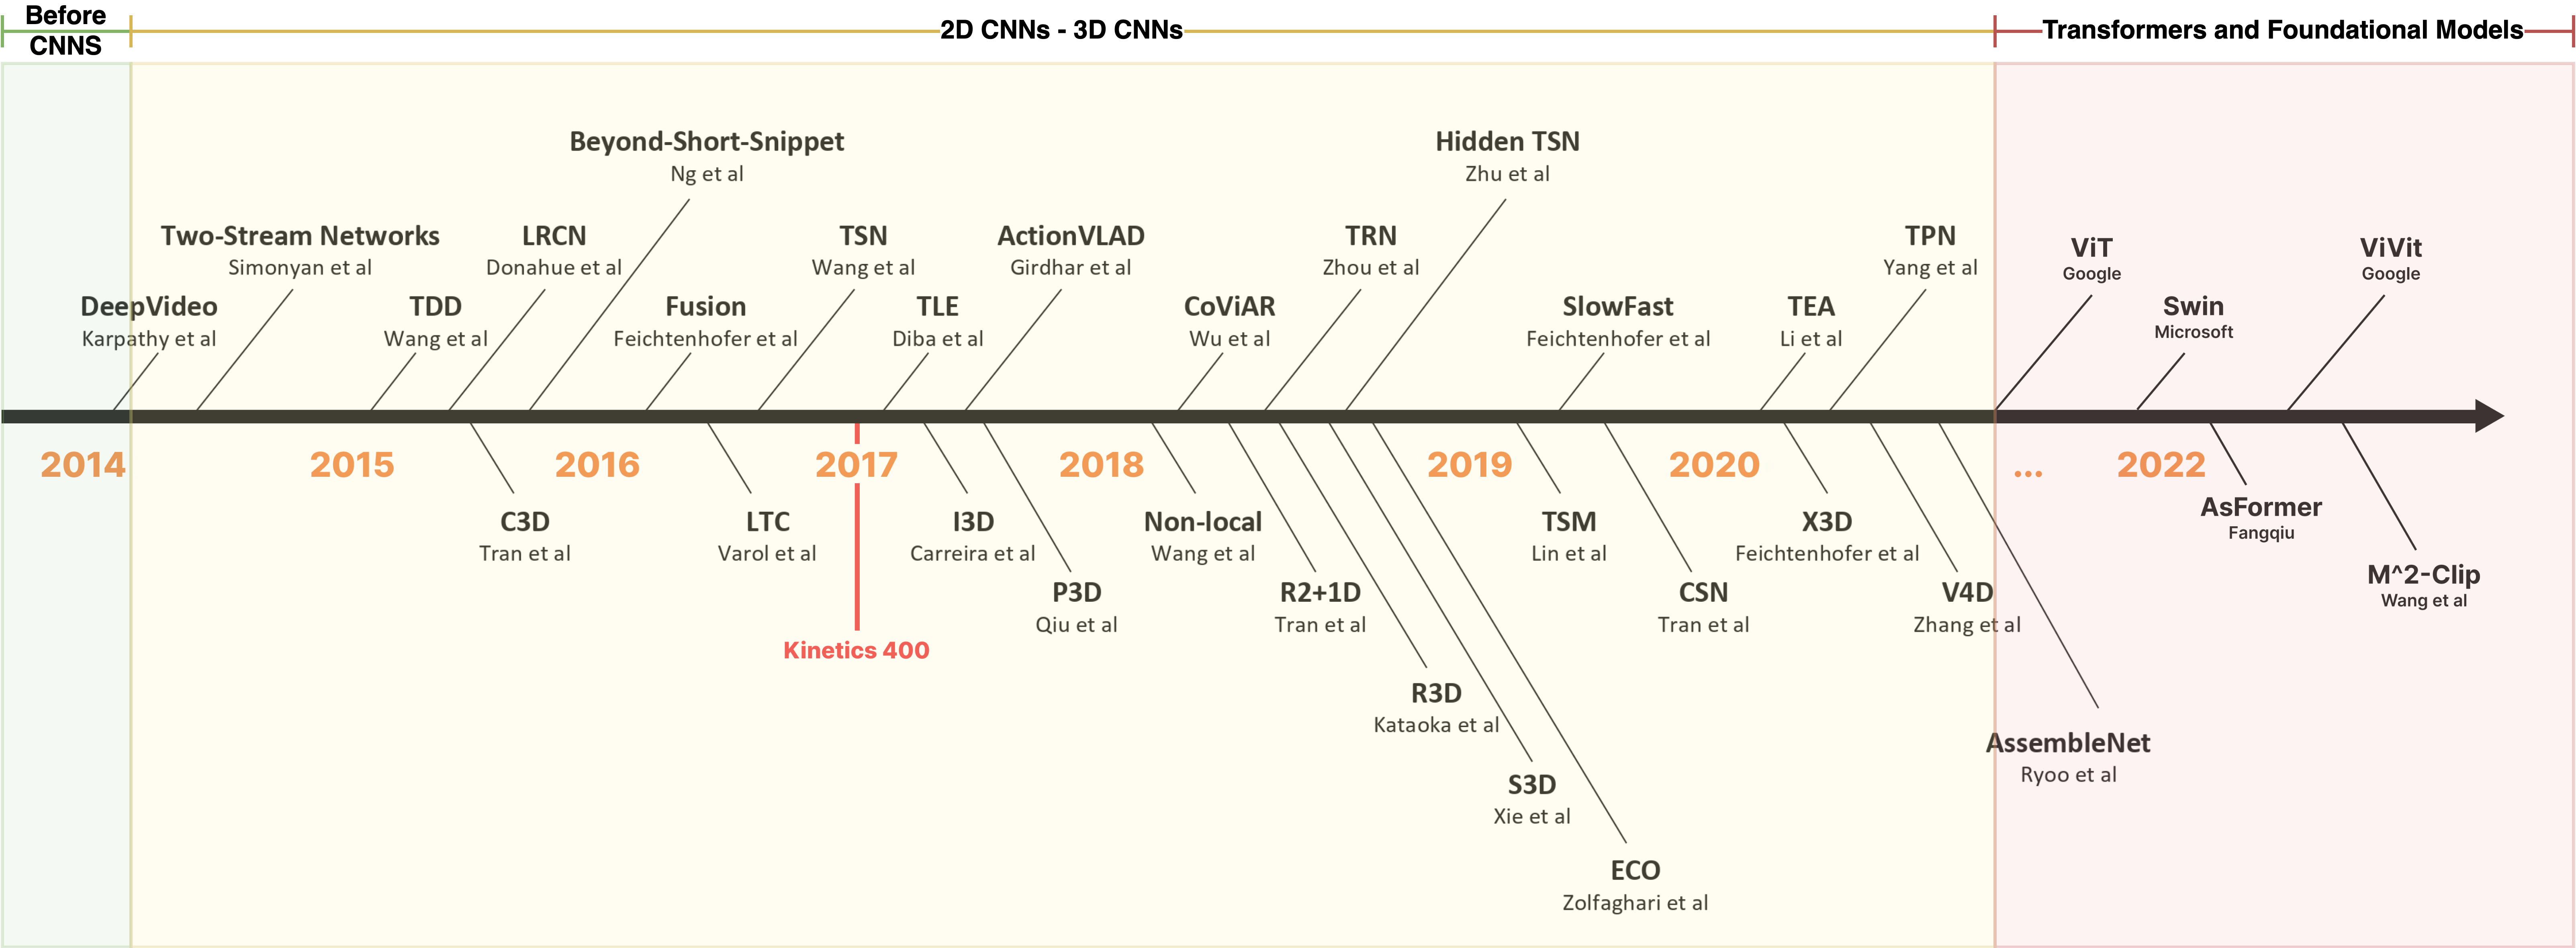
\includegraphics[width=\textwidth]{../../assets/figures/extended-video-timeline-v3.png}
    \caption{A timeline overview of the evolution of video analysis models.}
    \label{fig:your-label}
\end{figure*}

\section{Related Work}

In this section, we explore some of the prominent approaches to temporal action segmentation (TAS), discussing how methods have evolved over time as computational power and dataset availability have increased.

Compared to image and text data, video data is far more limited in terms of available datasets. While datasets such as Kinetics, Something-Something, and HowTo100M have significantly contributed to the field, video-based models are still more computationally expensive than their image or text counterparts. This high computational cost and the limited availability of large video datasets have contributed to the slower progress of video-related networks compared to other forms of data.

\subsection{The Evolution of Video Analysis Models}

The development of video analysis models has seen a significant shift as computational power and dataset size have increased. Initially, video analysis relied heavily on hand-crafted feature extraction, where specific features such as pixels were manually chosen or extracted. With the introduction of optical flow, models began incorporating motion information, improving their ability to understand temporal sequences in videos.

As 2D Convolutional Neural Networks (CNNs) gained popularity, they were applied to video data for feature extraction, showing promising results for action recognition. Following this, the introduction of 3D Temporal CNNs allowed for better understanding of the temporal dimension in videos. These methods, combined with the advent of larger datasets like Kinetics and Something-Something, marked a turning point in video action recognition, leveraging deep learning to handle complex temporal and spatial patterns in video data.

In recent years, transformers have also emerged as a promising approach for video analysis. Initially used for NLP tasks, transformers have demonstrated strong potential for video action recognition. However, unlike CNNs, transformers lack strong inductive biases, such as locality and translation invariance, which CNNs excel at. This makes transformers more dependent on massive amounts of data to perform effectively. Despite their growing popularity, transformers in video analysis are still less performant than their counterparts in text analysis, primarily due to the scarcity of large-scale video datasets.

The increasing availability of video datasets and computational resources has catalyzed these developments, enabling more sophisticated models. However, video models still face significant challenges due to the vast and diverse distribution of video data. This distribution causes models to drift more rapidly compared to other data types, which makes generalization across different datasets more difficult. Consequently, large datasets are essential for training video models, and pre-trained models often struggle to generalize beyond their original training sets.

\subsection{Temporal Action Segmentation and Its Approaches}

Temporal Action Segmentation can be approached in several ways. Here, we explore a few key perspectives:

\noindent\textbf{1. Video Classification.} In video classification, the focus is on assigning a single action label to an entire video or segment, typically using models such as 2D or 3D CNNs. This is the most popular perspective in the field, with well-established pre-trained networks available for various datasets. 

\noindent\textbf{2. Temporal Action Detection / Localization.} In this approach, the goal is to detect the temporal boundaries of actions within a video. This task is more challenging than video classification as it requires the model to identify both the start and end of actions while also classifying them.

It is important to note that while the above methods are highly computationally demanding and require large datasets, Temporal Action Segmentation (TAS) still plays a critical role in real-world applications, such as video surveillance, human-robot interaction, and activity recognition in videos.

\subsection{Challenges and Future Directions}

Video data presents a challenging problem due to its vast and diverse distribution, causing models to drift more rapidly compared to other data types. As a result, handling video data often requires significantly larger datasets. Even pre-trained models struggle to generalize well beyond their original training sets, making this an active area of ongoing research.

With the rise of computational power, the gap between text and video models has been closing. However, while transformers have shown great potential in video analysis, they are still behind their text counterparts in terms of performance. This discrepancy arises from the lack of inductive biases, like those present in CNNs, and the enormous quantity of data required to train transformers effectively. As more large-scale video datasets become available, we can expect transformers to become more viable for video analysis tasks, though they still demand considerable computational resources.